\documentclass[12pt,final]{amsproc}
\usepackage[top=2cm,bottom=3cm,left=3cm,right=2cm]{geometry}

\usepackage{amsmath}
\usepackage{amssymb}
\usepackage{amsthm}
\usepackage{listings}
%\usepackage{verbatim}
\usepackage{graphicx}
\usepackage{wrapfig}
\usepackage{tabularx}


\usepackage[backend=biber]{biblatex} % I try to use biber.
\bibliography{all} % the all.bib file

\linespread{1.3}
\sloppy

\makeatletter
\newcommand{\addresseshere}{%
  \enddoc@text\let\enddoc@text\relax
}
\makeatother
 
\usepackage{xltxtra}
\setmainfont[
Mapping=tex-text,
BoldItalicFont=arnamu_italic_bold.ttf,
BoldFont      =arnamu_bold.ttf,
ItalicFont    =arnamu_italic.ttf]{arnamu.ttf}

\renewcommand\figurename{Նկ․}
\renewcommand\tablename{Աղյուսակ}
\renewcommand\refname{Գրականություն}
\renewcommand\contentsname{Բովանդակություն}


\title{Հեբբյան ուսուցում}
\author{Հրանտ Խաչատրյան}
\address{Երևանի պետական համալսարան\\ Ինֆորմատիկայի և կիրառական մաթեմատիկայի ֆակուլտետ}
\email{hrant.khachatrian@ysu.am}
\date{Դեկտեմբերի 17, 2014}

\begin{document}
\maketitle
\addresseshere

\section{Ներածություն}\
Նեյրոճկունությունը (neuroplasticity)՝ ուղեղում նեյրոնների միջև կապերի փոփոխվելու հատկությունը, համարվում է ուղեղում ուսուցման պրոցեսի հիմնական մեխանիզմը \cite{doi:10.1146/annurev.neuro.27.070203.144216}: Նեյրոգիտության մեջ տարբերակում են ուղեղի սինապտիկ և ոչ սինապտիկ ճկունություն: Սինապտիկ ճկունությունը նեյրոնների միջև սինապսների ուժեղացումն ու թուլացումն է, իսկ ոչ սինապտիկ ճկունությունը աքսոններում, դենդրիտներում, ինչպես նաև բջջի մարմնում կատարվող կենսաքիմիական փոփոխություններն են, որոնք փոխում են նեյրոնի էլեկտրական հատկությունները: Սինապտիկ ճկունությունը կարող է լինել կարճաժամկետ (մի քանի վայրկյան) և երկարաժամկետ (րոպեներ և ավել): Կանադացի հոգեբան Դոնալդ Հեբբը 1949թ․ առաջարկեց երկարաժամկետ սինապտիկ ճկունության քանակական տեսություն \cite{Hebb194912}, որը հաճախ ձևակերպվում է մեկ կանխադրույթով․ «միաժամանակ գրգռվող նեյրոնները կապվում են միմյանց»: Այս սկզբունքը հետագայում զարգացվեց՝ վերածվելով ավելի բարդ մաթեմատիկական մոդելների, որոնցից օրինակ BCM տեսությունը հաջողությամբ նկարագրում է ուղեղի որոշ հատվածներում (տեսողական կեղև, հիպոկամպ) նեյրոնների վարքը և հաստատվել է մի շարք փորձարարական փաստերով \cite{CooperIntratorBlaisShouval200404}: 

Համակարգչային գիտություններում մի շարք կիրառական խնդիրների լուծման գործում մեծ դեր են խաղում կենսաբանական մեխանիզմներից ներշնչված արհեստական նեյրոնային ցանցերը: Մասնավորապես, ձայնի և պատկերների ճանաչման խնդիրներում ամենաարդյունավետ ծրագրերից շատերը հիմնված են այսպես կոչված խորը նեյրոնային ցանցերի վրա, որի տեսական հիմքերը տանում են մինչև Հեբբյան տեսություն: Այս աշխատանքի նպատակն է նկարագրել սինապտիկ ճկունության Հեբբյան և նրանից ածանցյալ տեսությունները, ինչպես նաև նրանց ազդեցությունը արհեստական նեյրոնային ցանցերի նախագծման վրա: 

\section{Հեբբյան տեսություն}

\begin{figure}[b!]
\centering
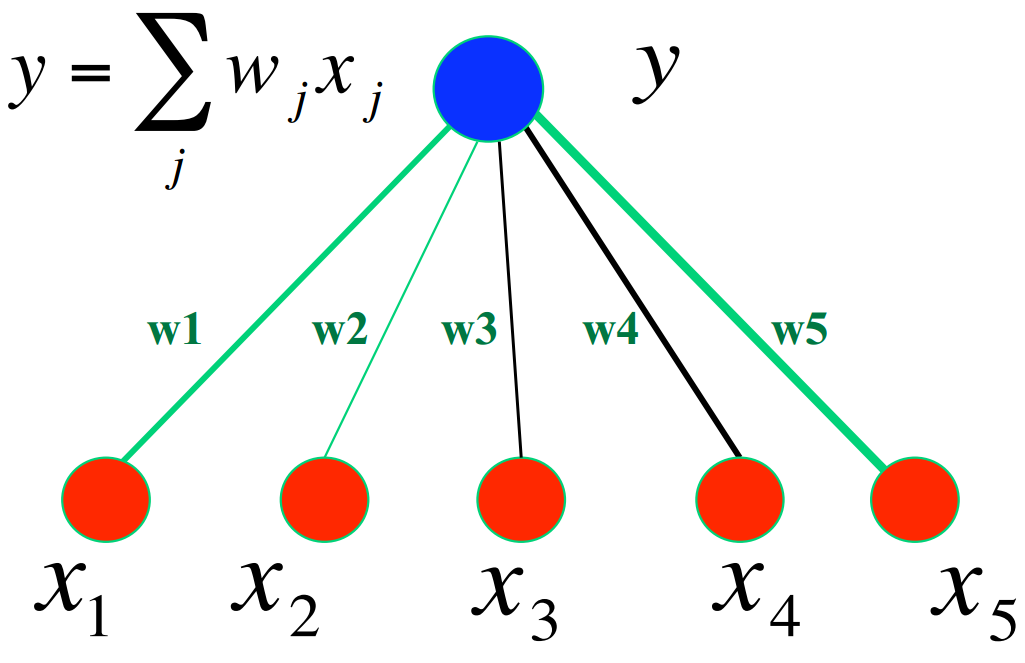
\includegraphics[width=0.5\textwidth]{neuron.png}
\caption{Նեյրոնի գրգռման մոդելավորումը գրաֆի միջոցով \cite{BCMSlides}}
\label{neuron}
\end{figure}

Նեյրոնների գրգռման պրոցեսը կարելի է մոդելավորել գրաֆի միջոցով, որտեղ գրաֆի գագաթները նեյրոններն են, իսկ կողերը՝ սինապսները: Դիցուք $n$ նեյրոնների աքսոնները միանում են մի նեյրոնի (Նկ․ \ref{neuron}): $x_j$-ով նշանակվում է $j$-րդ սինապսի նախասինապսային նեյրոնի ակտիվությունը, իսկ $y$-ով՝ հետսինապսային նեյրոնի ակտիվությունը: Հաճախ ընդունվում է, որ հետսինապսային ակտիվությունը հավասար է նախասինասպային ակտիվությունների գումարին՝ կշռված սինապսների $w_j$ կշիռներով (այս դեպքում նեյրոնը կոչվում է \textit{գծային նեյրոն}):
\begin{center}
$y=\sum\limits_{j=1}^{n}w_jx_j$
\end{center}

Սինապսային ճկունությունը կայանում է նրանում, որ սինապսների կշիռները ժամանակի ընթացքում փոխվում են: Դոնալդ Հեբբը իր \textit{The Organization of Behavior} \cite{Hebb194912} գրքում առաջարկեց սինապսների ուժգնության այդպիսի փոփոխությունները նկարագրող տեսություն: Ըստ նրա, եթե A նեյրոնի աքսոնը պարբերաբար մասնակցում է B նեյրոնի գրգռմանը, ապա այդ նեյրոններում տեղի են ունենում որոշակի փոփոխություններ, որոնց արդյունքում B նեյրոնի գրգռման գործում A նեյրոնի արդյունավետությունը մեծանում է: Այս փաստը կարելի է մոդելավորել հետևյալ կերպ․ սինապսային ուժգնության փոփոխությունը համեմատական է նախասինապսային ակտիվությանը: Հաճախ դա գրվում է այսպես․
\begin{center}
$\frac{dw_i}{d_t}=\eta x_i y$
\end{center}
որտեղ $\eta$-ն ուսուցման արագությունն է: Այս պարզունակ մոդելը ունի մի շարք թերություններ: Մասնավորապես, այն թույլ է տալիս սինապսների անվերջ ուժեղացում և կայուն չէ: Այս խնդիրը լուծելու համար առաջարկվել են Հեբբի մոդելի մի շարք ընդհանրացումներ: 

\subsection{Օյայի կանոն}
Ֆինն մաթեմատիկոս Էրկի Օյան 1982թ․ առաջարկեց Հեբբի մոդելին ավելացնել որոշակի նորմավորում, ինչը թույլ տվեց լուծել կայունության խնդիրը \cite{Oja}: Օյայի կանոնը գրվում է հետևյալ կերպ․
\begin{center}
$\frac{dw_i}{d_t}=\eta y (x_i - yw_i)$
\end{center}
Ապացուցվում է, որ այս օրենքով աշխատող համակարգը կայուն է և սինապսների ուժգնությունը անվերջ չի աճում:

\subsection{BCM տեսություն}

\begin{figure}[b!]
\centering
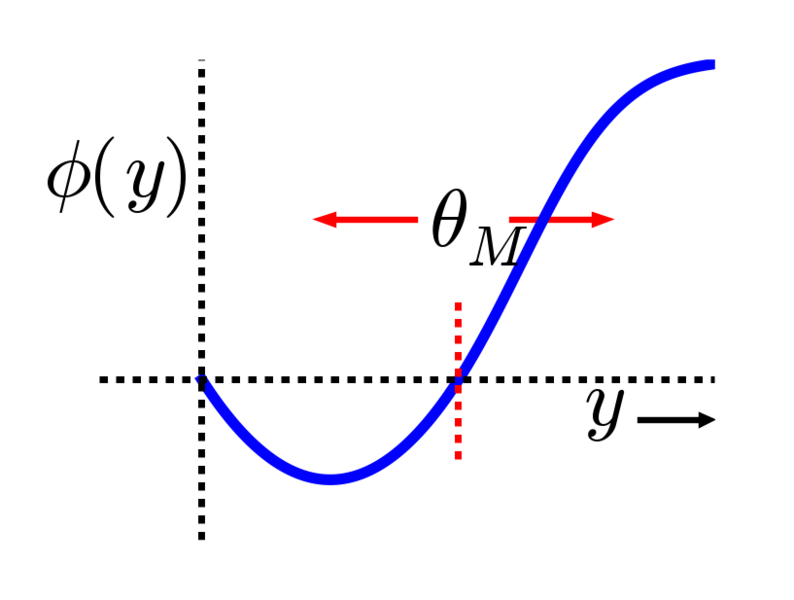
\includegraphics[width=0.6\textwidth]{bcm.png}
\caption{Սինապսի ուժգնության փոփոխության կախումը նեյրոնի գրգռման աստիճանից \cite{BCMScholarpedia}}
\label{BCM}
\end{figure}

Հեբբի մոդելի մեկ այլ ընդհանրացում առաջարկվեց Բինենստոկի, Կուպերի և Մունրոյի կողմից 1982թ․ \cite{BCM1982}: Ուսումնասիրելով կենդանիների տեսողական կեղևի մասին հայտնի փորձարարական տվյալները նրանք առաջարկեցին հետևյալ երեք կանխադրույթները․
\begin{enumerate}
\item Սինապսի կշռի $dw_i/dt$ փոփոխությունը համեմատական է $x_i$ նախասինապսային ակտիվությանը
\item Սինապսի կշռի փոփոխությունը համեմատական է $y$ հետսինապսային ակտիվությունից կախված ոչ գծային և ոչ մոնոտոն ֆունկցիայի՝ $\phi(y, \theta_M)$: Այս ֆունկցիան կախված $\theta_M$ \textit{փոփոխման շեմից} կարող է լինել բացասական (երբ հետսինապսային ակտիվությունը թույլ է՝ $y < \theta_M$) կամ դրական (երբ $y > \theta_M$, Նկ․ \ref{BCM})
\item $\theta_M$ փոփոխման շեմը իր հերթին կախված է հետսինապսային ակտիվության պատմությունից:
\end{enumerate}

Այս սկզբունքներին բավարարող բազմաթիվ մաթեմատիկական մոդելներ կան, օրինակ․
\begin{align*}
y &= \sum\limits_{i}{w_ix_i} \\
\frac{dw_i}{d_t} &= x_i \phi(y_i, \theta_M) - \epsilon w_i \\
\theta_M &= E[(y/y_0)]
\end{align*}

Հեղինակները իրենց առաջին հոդվածում որպես $\phi(y, \theta_M)$ ֆունկցիա վերցնում էին $y(y-\theta_M)$: Հետագայում առաջարկվել են մի շարք այլ մոտեցումներ ևս \cite{BCMScholarpedia}: BCM մոդելի կայունությունը ապահովվում է փոփոխվող $\theta_M$ շեմի միջոցով, որը հավասար է ժամանակի ընթացքում հետսինապսային ակտիվության միջին արժեքին (որոշ մոդելներում՝ նորմավորված որևէ $y_0$ հաստատունով): Սինապսի ուժգնության փոփոխությանը մասնակցում է նաև $- \epsilon w_i$ գումարելին, ինչը ապահովում է նեյրոնների ակտիվության բացակայության ժամանակ սինապսի ուժգնության հավասարաչափ թուլացում $\epsilon$ արագությամբ:

\section{Արհեստական նեյրոնային ցանցեր}

\begin{figure}[b!]
\centering
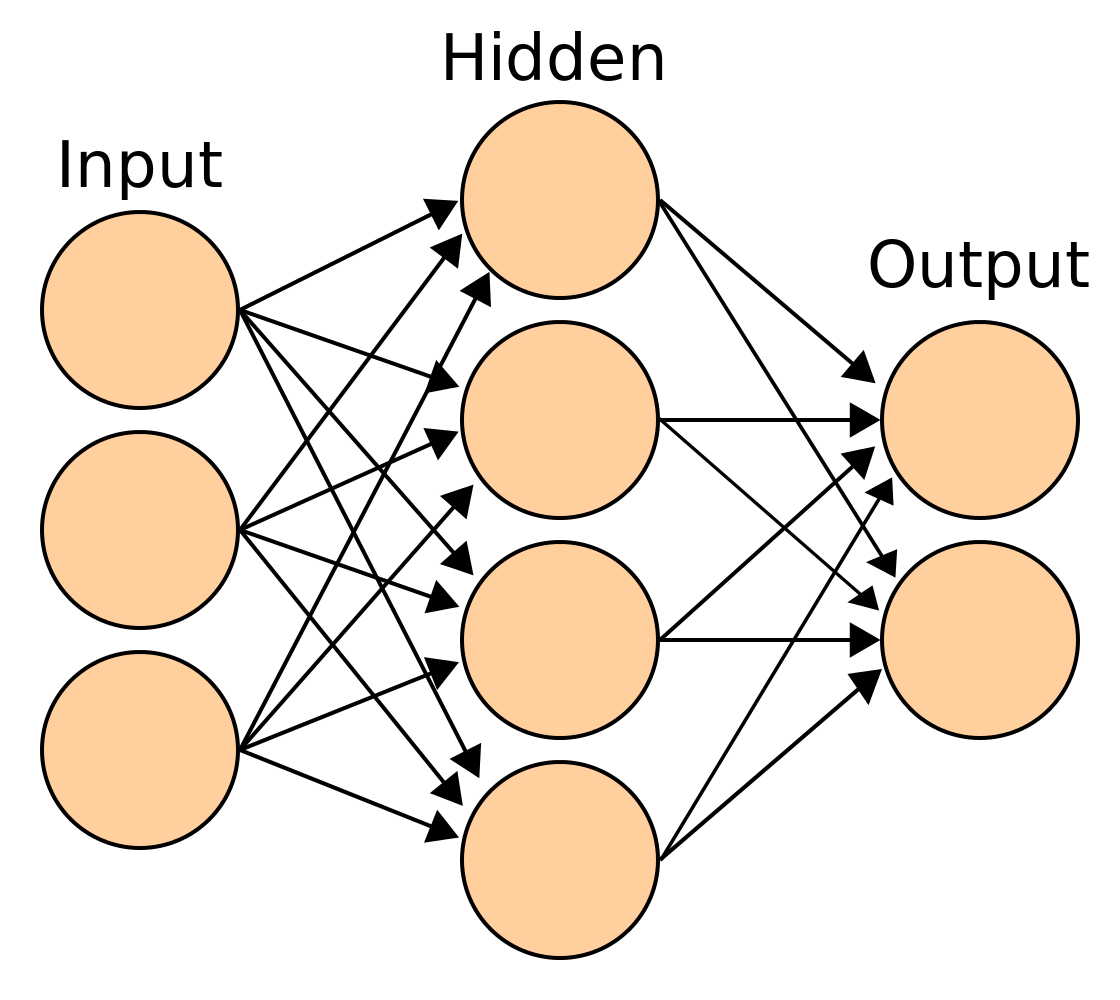
\includegraphics[width=0.5\textwidth]{ann.png}
\caption{Պարզագույն նեյրոնային ցանց. ձախ շարքում մուտքի նեյրոններն են, մեջտեղում՝ թաքնված շերտը, աջ շարքում՝ ելքի նեյրոնները \cite{WikiANNImage}}
\label{ANN}
\end{figure}

Արհեստական նեյրոնային ցանցերը մեքենայական ուսուցման ալգորիթմներ են՝ ներշնչված կենսաբանական նեյրոնային ցանցերից: Նեյրոնային ցանցը կազմված է մի քանի շերտ դասավորված նեյրոններից: Առաջին շերտի նեյրոնները կոչվում են մուտքի նեյրոններ և նրանց գրգռումը ուղղակիորեն կախված է ալգորիթմի մուտքից: Օրինակ, պատկերների ճանաչման մի շարք խնդիրներում պատկերը ներկայացվում է երկուական մատրիցի տեսքով, որտեղ պատկերի ամեն մի կետը (պիքսելը) ներկայացվում է որպես զրո կամ մեկ: Ամեն կետին համապատասխանեցվում է մի նեյրոն, որը գրգռվում է, եթե կետի արժեքը հավասար է մեկի: Հաջորդ շերտերի նեյրոնները գրգռվում են կախված նախորդ շերտի նեյրոնների վիճակից և նախորդ շերտի հետ ունեցած կապերի ուժգնությունից: Նեյրոնային ցանցի ուսուցման պրոցեսում այդ կապերի ուժգնությունը փոխվում է: Վերջին շերտի նեյրոնները կոչվում են ելքի նեյրոններ և նրանց վիճակը ալգորիթմի աշխատանքի վերջում հանդիսանում է ալգորիթմի ելքը: Օրինակ, թվանշանների ճանաչման համար նախատեսված նեյրոնային ցանցի վերջին շերտում սովորաբար լինում են տաս նեյրոններ, որոնցից յուրաքանչյուրը համապատասխանում է մի թվանշանի: Այսպիսով, արհեստական նեյրոնային ցանցերը տրվում են ըստ երեք պարամետրերի \cite{WikiANN}.

\begin{enumerate}
\item Նեյրոնների միջև եղած կապեր՝ ցանցի հիմքում ընկած գրաֆը: Երբ գրաֆը ուղղորդված է և ցիկլ չի պարունակում, գործ ունենք feedforward նեյրոնային ցանցերի հետ: Երբ ցանցում կան ցիկլեր, այն կոչվում է անդրադարձ (recurrent) ցանց
\item Ուսուցման պրոցես, ըստ որի փոփոխվում են նեյրոնների միջև եղած կապերի ուժգնությունը
\item Ակտիվացման ֆունկցիա, ըստ որի նեյրոնի ստացած մուտքի համաձայն որոշվում է նեյրոնի գրգռման աստիճանը
\end{enumerate}

Հեբբյան ուսուցման վրա հիմնված նեյրոնային ցանց ստեղծվեց արդեն 1953թ․ \cite{FarleyClark1954}: Սակայն կիրառական խնդիրների լուծման գործում մեծ հաջողությունների հասնել երկար ժամանակ չէր հաջողվում, քանի որ պահանջվող հաշվարկները չափազանց բարդ էին գոյություն ունեցող համակարգիչների համար: 1990-ականներին մեքենայական ուսուցման այլ մեխանիզմների հաջողությունները (support vector machines, linear classifiers) ժամանակավորապես դուրս մղեցին նեյրոնային ցանցերին կիրառություններից \cite{WikiANN}:

\subsection{Խորը նեյրոնային ցանցեր}
Պարզագույն նեյրոնային ցանցերը բացի մուտքի և ելքի նեյրոններից ունեն միայն մեկ շերտ նեյրոններ: Դա հնարավորություն չի տալիս նեյրոնային ցանցին սովորել բարդ կառուցվածքներ առանց նեյրոնների թվի զգալի մեծացման: Այս խնդիրը լուծելու համար 1990-ականներին սկսեցին դիտարկել մեկից ավելի միջանկյալ շերտերով նեյրոնային ցանցեր, որոնք կոչվեցին խորը նեյրոնային ցանցեր (deep neural networks): Սակայն այս համակարգերը արդյունավետությամբ զիջում էին մեքենայական ուսուցման այլ համակարգերին տեխնիկական պատճառներով: 

Խորը նեյրոնային ցանցերի զարգացման պատմությունը մանրամասն շարադրված է Շմիդհուբերի 2014թ․ հրապարակված հոդվածում \cite{DBLP:journals/corr/Schmidhuber14}: Վերջին տարիներին մի շարք տեսական նվաճումների, ինչպես նաև համակարգիչների արագործության մեծացման շնորհիվ, այսպիսի նեյրոնային ցանցերով աշխատող համակարգերը արդյունավետությամբ շրջանցեցին գոյություն ունեցող բոլոր այլ համակարգերին մի շարք ոլորտներում (խոսքի ճանաչում, մարդու դիրքի որոշում, պատկերների ճանաչում և այլն):

\subsection{Թվանշանների ճանաչում}

\begin{figure}[b!]
\centering
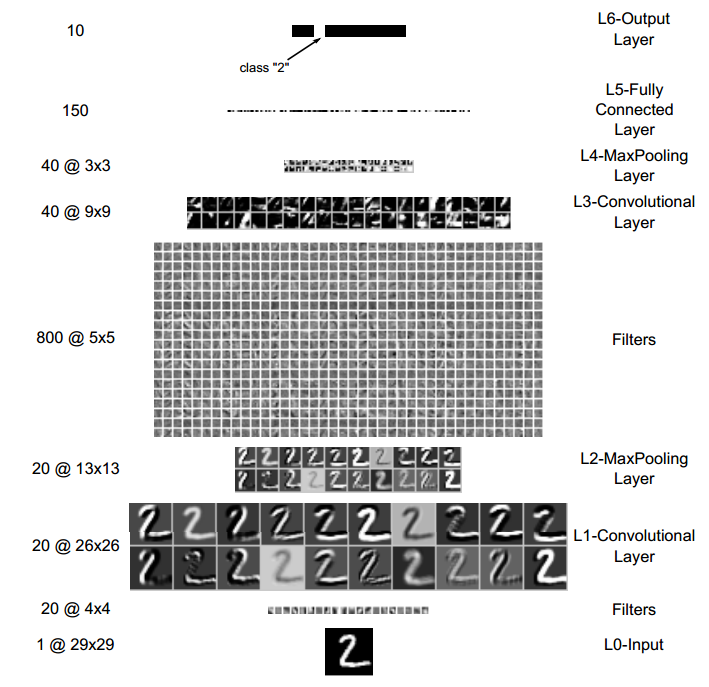
\includegraphics[width=0.85\textwidth]{mnist-dnn.png}
\caption{Ձեռագիր թվանշաններ ճանաչող նեյրոնային ցանցի սխեմատիկ նկարագրությունը \cite{MNIST023} հոդվածից}
\label{MNIST-DNN}
\end{figure}

Ձեռագիր թվանշանների ճանաչման տարբեր ալգորիթմների համեմատության համար ստեղծվել է թվանշանների պատկերների MINST տվյալների բազան \cite{MNIST}: Այն պարունակում է 60000 պատկեր մեքենային ուսուցանելու համար և ևս 10000 պատկեր ծրագրի աշխատանքը ստուգելու համար: Թվանշանները գրված են ԱՄՆ պետական աշխատողների և ուսանողների կողմից: Բոլոր պատկերները նորմալիզացված չափերի են՝ 20x20 կետայնությամբ և գունավոր չեն: 2010թ․ խորը նեյրոնային ցանցի հիման վրա աշխատող ծրագիրը կարողացավ հասնել 99.65\% ճշտության, հաշվարկները կատարելով  գրաֆիկական պրոցեսորների վրա \cite{MNIST035}: 2014թ․ դեկտեմբերի դրությամբ լավագույն արդյունքը պատկանում է նույն հեղինակներին՝ 99.77\% ճշտություն \cite{MNIST023}: Համարվում է, որ մարդը ձեռագիր թվանշանները ճանաչում է մոտ 99.8\% ճշտությամբ: Այս վերջին հոդվածում հեղինակները նկարագրում են նման նեյրոնային ցանցերի աշխատանքը մի շարք այլ խնդիրների համար ևս, ինչպես օրինակ լատիներեն և չինարեն տառերի ճանաչում, ճանապարհային նշանների ճանաչում, եռաչափ պատկերի ճանաչում լուսանկարում: Բոլոր այս խնդիրներում ներկայացվող ծրագրերը գրանցել են ճանաչման ճշտության նոր ռեկորդներ:

\subsection{Տեսական արդյունքներ խորը նեյրոնային ցանցերի վերաբերյալ}

Գործնականում գրանցված հաջողություններից միայն մի քանի տարի անց, 2013թ․, ստացվեցին խորը նեյրոնային ցանցերի արդյունավետության առաջին տեսական հիմնավորումները: \cite{Arora2013}-ում նկարագրվեց խորը ուսուցման ալգորիթմ, որի արդյունավետությունը ապացուցվեց տեսական ճանապարհով, հաշվարկվեց ալգորիթմի բարդությունը և այլն: Հեղինակների պնդմամբ, առաջարկված ալգորիթմը հետևում է Հեբբի կանոնին, հետևյալ մեկնաբանությամբ․ «միևնույն շերտում գտնվող միաժամանակ գրգռվող նեյրոնները մեծ հավանականությամբ կապված են հաջորդ բարձր շերտի միևնույն նեյրոնին»: Ալգորիթմի աշխատանքի ընթացքում հայտնաբերվում են այսպես կորելացված նեյրոնների զույգերը և դրանց միջոցով վերականգնվում է ամբողջ նեյրոնային ցանցը: Դա բերվում է հայտնի խնդրի մաթեմատիկայից (գրաֆների տեսությունից)՝ երկկողմանի գրաֆի վերականգնումը երկու հեռավորության վրա գտնվող գագաթների զույգերից: Վատագույն դեպքում այս խնդիրը NP-լրիվ է, սակայն նոսր պատահական գրաֆների համար կառուցվում է բազմանդամային ալգորիթմ: 

\subsection{Օբյեկտների ճանաչում լուսանկարից}

\begin{figure}[b!]
\centering
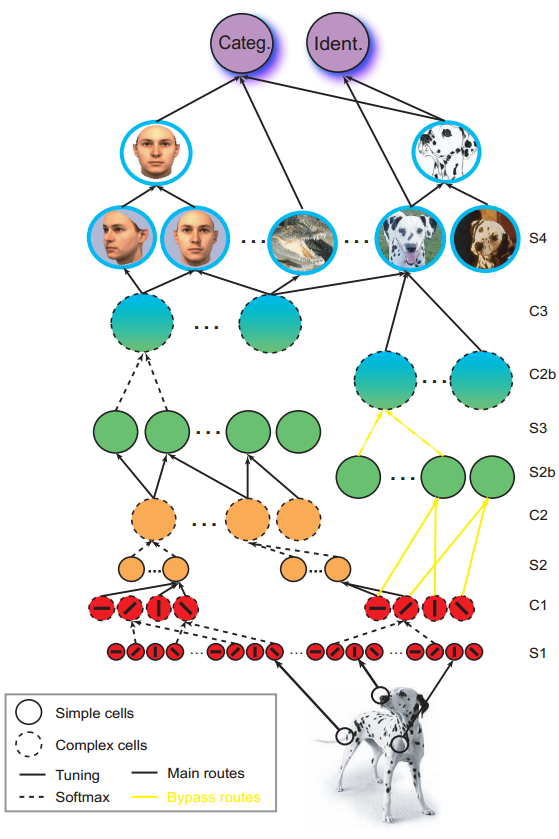
\includegraphics[width=0.75\textwidth]{serre2005.PNG}
\caption{Տեսողական կեղևում օբյեկտի ճանաչման սխեման ըստ \cite{Serre2005} աշխատանքում նկարագրված տեսության: Առաջին շերտերի նեյրոնները ճանաչում են պարզագույն կառուցվածքները (գծեր, կորեր), ավելի բարձր շերտերի նեյրոնները ճանաչում են ավելի բարդ կառուցվածքներ}
\label{Serre2005Fig}
\end{figure}

Մեքենայական ուսուցման ամենաբարդ խնդիրներից մեկը լուսանկարներից օբյեկտների ճանաչումն է: Այսպիսի ծրագրերի համեմատության համար 2010թ․ ամեն տարի Սթենֆորդի համալսարանը անցկացնում է ImageNet Large Scale Visual Recognition Challenge մրցույթը: 2014թ․ մրցույթի համար հավաքվել էին մոտ 1.2 միլիոն լուսանկարներ վարժեցման համար (հիմնականում Flickr կայքից), որոնցից յուրաքանչյուրի մեջ նշվել էին երևացող օբյեկտները թվով 1000 կատեգորիաներից: Դրվում են մի քանի խնդիրներ, օրինակ՝ դասակարգել 100000 նոր լուսանկարներ նույն 1000 կատեգորիաներում: 2014թ․ մրցույթում լավագույն արդյունքը ցուցադրեց Google ընկերության աշխատակիցների ստեղծած GoogLeNet ծրագիրը: Ծրագիրը յուրաքանչյուր լուսանկարի համար նշում է հինգ կատեգորիաներ, որոնց պետք է պատկանի այդ լուսանկարը: GoogLeNet-ը այս չափանիշով ունեցավ 93.33\% արդյունավետություն (2013թ․ լավագույն ցուցանիշը 88.8\% էր): Ծրագիրը օգտագործում է 22 շերտ ունեցող խորը նեյրոնային ցանց, որի աշխատանքը մանրամասն նկարագրված է հեղինակների աշխատանքում \cite{GoogLeNet2014}: Մասնավորապես նրանք նշում են, որ հիմնվել են \cite{Arora2013} աշխատանքում կատարված տեսական աշխատանքի վրա, այսպիսով իրենց ծրագիրը կապելով Հեբբյան մոդելներին:

 
GoogLeNet-ի հիմքում ընկած են նեյրոգիտության այլ նվաճումներ ևս: 2005թ․ \cite{Serre2005}-ում առաջարկվել է պրիմատների տեսողական կեղևի մի հատվածում (ventral stream) տեղի ունեցող օբյեկտների ճանաչման պրոցեսի քանակական տեսություն, որը համապատասխանում է օբյեկտի նախնական ճանաչման փուլին: Այդ փուլը տեղի է ունենում ճանաչման առաջին 150մվ ընթացքում, երբ ուղեղի այլ հատվածներից եկող ազդակները (top-down signals) դեռևս դեր չեն խաղում ճանաչման համար: Հեղինակները պնդում են որ այս փուլում են կատարվում օբյեկտների դասակարգման հիմնական քայլերը: 

Այս տեսության հիման վրա \cite{Serre2007}-ում ստեղծվել է պատկերների ավտոմատ ճանաչման համակարգ: Այս համակարգի կարևորագույն հատկությունը, ինչպես նշում են GoogLeNet-ի հեղինակները, օբյեկտների ճանաչման կարողությունն է անկախ նրանց մասշտաբից և ուղղությունից: GoogLeNet-ում ևս կիրառվել են այդ մեթոդները, սակայն ոչ թե նեյրոնային ցանցի երկու շերտերով, ինչպես \cite{Serre2007}-ում, այլ միանգամից 22: 

\section*{Եզրակացություն}
Վերջին տասնամյակներում նեյրոգիտության նվաճումների արդյունքում զգալիորեն ընդլայնվել են պատկերացումները մարդու ուղեղի աշխատանքի վերաբերյալ: Ի հայտ են գալիս քանակական տեսություններ, որոնք փորձում են բացատրել ուղեղի այս կամ այն հատվածի աշխատանքը: Համակարգչային գիտությունների ներկայացուցիչները հետևելով այս զարգացումներին կարողանում են ստեղծել ուղեղում ընթացող պրոցեսները նմանակող արհեստական նեյրոնային ցանցեր, որոնց արդյունավետությունը գերազանցում է գոյություն ունեցող մեքենայական ուսուցման այլ համակարգերին բազմաթիվ կիրառական խնդիրների համար: Նեյրոնային ցանցերը սկսում են օգտագործվել ոչ միայն դասակարգման կամ ճանաչման խնդիրներում: Այսպես, 2014թ․ դեկտեմբերին Google ընկերության Deep Mind թիմը հայտարարեց նեյրոնային ցանցով աշխատող մի ծրագրի մասին, որը կարողանում է սովորել իրականացնել պարզագույն ալգորիթմներ, ինչպես օրինակ տվյալների արտագրում կամ սորտավորում \cite{NTM}: \cite{Go} աշխատանքում նկարագրված է, թե ինչպես են խորը նեյրոնային ցանցերը օգտագործվում Գո սեղանի խաղի համար (որի դեպքում, ի տարբերություն շախմատի, լավագույն խաղացողները դեռևս հեշտությամբ հաղթում են համակարգչային ծրագրերին): 

Ամեն տարի անցկացվող Neural Information Processing Systems գիտաժողովում ներկայացվող աշխատանքներում խորը նեյրոնային ցանցերի մասին աշխատանքների քանակը աճում է տարեկան մոտ երկու անգամ: Ոլորտի նկատմամբ հետաքրքրությունը աճում է չափազանց մեծ տեմպերով, և չնայած նեյրոնային ցանցերը շարունակում են նոր հաջողություններ գրանցել տարբեր կիրառական խնդիրներում, անհրաժեշտություն կա կատարել նաև տեսական բնույթի աշխատանքներ՝ մեթոդների կիրառելիության սահմանները հասկանալու համար:

\printbibliography[title={Գրականություն}]

\end{document}